\section{Experimentación y análisis}

\subsection{De Nueva York a Oxford}

Dado que existe un paralelísmo geográfico que acompaña a nuestro análisis, decidimos buscar algo para ejemplificarlo de manera visual. Elegimos la herramienta \textit{IP Fingerprints}\footnote{http://www.ipfingerprints.com/} que nos permite graficar, de forma aproximada, la ubicación de las máquinas por las que se pasa en la ruta, dándonos además, sus coordenadas; y con ellas, la posibilidad de ver en el mapa a dónde corresponden las mismas.\\
\\
\indent Sabemos que de Nueva York a Oxford hay un cambio de continente en el medio, y eso equivale a al menos un pasaje por un enlace submarino. Como vista general, la ruta aproximada es la siguiente:
\begin{center}
	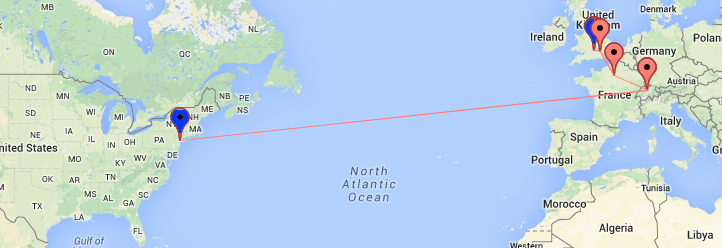
\includegraphics[scale=0.6]{graphics/new_york-oxford.png}
\end{center}

Tal y como lo sospechábamos, podemos observar enlaces internos en Estados Unidos y enlaces internos en Europa, unidos por un gran enlace submarino entre ambos continentes. Decidimos distinguir los nodos de comienzo (en Nueva York) y fin de la ruta (en Oxford) pintándolos de color azul.\\
\\
\indent Viendo un poco más en detalle dentro de Nueva York, esta herramienta nos permitió ver que el primer hop es dentro de la ciudad de Nueva York, como vemos en esta imagen aumentada de la zona:

\begin{center}
	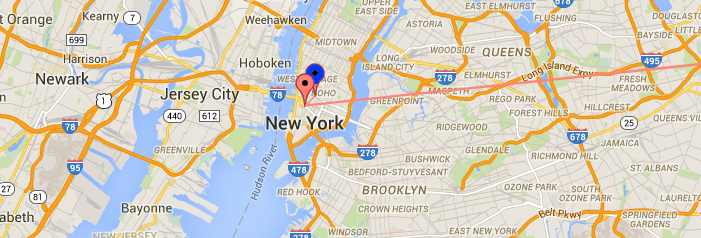
\includegraphics[scale=0.6]{graphics/new_york_zoom.png}
\end{center}

Una vez que sale de ahí, viaja por enlace submarino a Europa. Más precisamente, a Suiza, como se ve en la siguiente imagen aumentada de la zona:

\begin{center}
	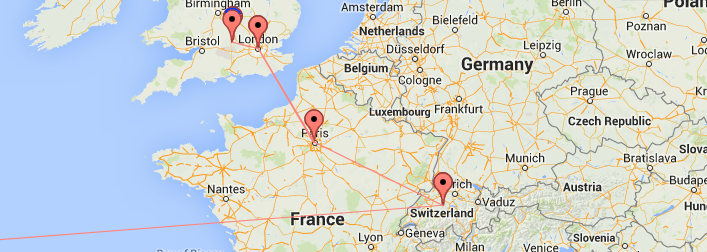
\includegraphics[scale=0.6]{graphics/europe_zoom.png}
\end{center}

Ahí envía paquetes en el mismo país unas 4 veces, hasta que sale y va a Francia, donde se envían 2 paquetes dentro de ese mismo país. Finalmente, de ahí pasa a la isla del Reino Unido, como vemos en la siguiente imagen:

\begin{center}
	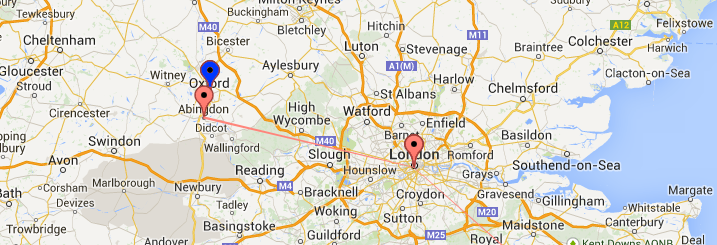
\includegraphics[scale=0.6]{graphics/united_kingdom_zoom.png}
\end{center}

Llega a Lóndres, envía 4 paquetes dentro de la ciudad, para luego ir a la ciudad donde finaliza el camino: Oxford. Ahí llega a la Universidad de Oxford, que es nuestro objetivo, salta a través de 3 máquinas, hasta efectivamente llegar a la que hostea el sitio web de la universidad.